\chapter{\dunyazad/}

\label{ch:dunyazad}%

As stated in the introduction, \dunyazad/ has two purposes as a project: first, to produce a \emph{system}, and second, to produce a \emph{theory}.
%
The system is a novel story generator that is focused on generating interesting choices, and on providing fine-grained control over the kinds of choices it uses.
%
The theory is a theory of choice poetics: a theory about how specific choice structures give rise to certain feelings, such as regret.
%
In order to satisfy these two goals, \dunyazad/ uses an answer set solver to turn a logical criteria for a certain kind of choice into an instance of such a choice---this is its core operating principle.


\dunyazad/'s code therefore largely consists of a set of logical statements describing what a choice structure is and when choices fit into one of several categories.
%
For example, there are statements that define a ``relaxed'' choice.
%
Answer sets for these rules are found using Potassco Labs' \clingo/ solver \citep{Gebser2011}.
%
Besides these rules, there is an external control structure which invokes the solver repeatedly, generating multiple choices and connecting them into a story.\footnote{
The model for \dunyazad/'s output is the Choose-Your-Own-Adventure book.
%
These books are young-adult novels which contain explicit choices: at the end of certain pages, the reader is instructed to choose an action for the protagonist, and continue reading at one of several different pages depending on their choice.
%
This combination of traditional linear narrative with intermittent discrete choices is one of the most straightforward examples of what I call ``choice-based narrative.''
%
Note that in contrast to Choose-Your-Own-Adventure books, choices in \dunyazad/ are separated by only a few sentences, rather than pages of text.}
%
The focus of development so far has been on individual choices, but the capacity exists for \dunyazad/ to generate a full branching story.
%
Of course, there is also some imperative code for turning a logical choice structure into English text, in the form of a template-based generation system.
%
The English-generation code and the control code are both written in Python.


The goal of this chapter is to describe in detail how \dunyazad/ functions.
%
First, \cref{sec:dunyazad-asp-and-ctp} describes why \dunyazad/ uses answer set programming in a bit more detail, and how answer set programming (ASP) helps with the theory development goal.
%
\Cref{sec:dunyazad-choice-generation} then describes how \dunyazad/ generates individual choices, while \cref{sec:dunyazad-control} describes the higher-level control mechanism.
%
Finally, \cref{sec:dunyazad-summary} summarizes the entire system and works through an example of how \dunyazad/ generates a choice from beginning to end.
%
Note that the template-based English generation system is described separately in \cref{ap:nlg}.

%\section{Goals}

\section{ASP and Critical Technical Practice}
\label{sec:dunyazad-asp-and-ctp}%

The idea of critical technical practice started as a call for technical practitioners (and especially AI researchers) to be more aware of the limits placed on their technical approaches by the central metaphors of their fields.
%
In Phil Agre's 1997 \work{Computation and Human Experience} he describes a process of critical examination to identify core metaphors and what those core metaphors marginalize, followed by an inversion that makes those marginalized concepts central \citep{Agre1997}.
%
This process can be used to drive innovation and find hidden limitations in a technical field by scrutinizing it using the tools of critical theory.


One common AI practice identifies a motivating theory from another discipline and then attempts to build a system that faithfully operationalizes that theory, taking the theory for granted as a known truth.
%
In contrast, critical technical practice seeks to question common assumptions (in particular through the application of critical theory) and then embark upon technical projects that use non-standard assumptions, thereby broadening the technical field.
%
\dunyazad/ as a project pursues a different relationship between theory and practice by seeing its driving theory (choice poetics) as both a \emph{product} of technical practice and a precursor to it, integrating theory development tightly with system development so that both the theory and the system are developed in dialogue with each other.
%
\dunyazad/ thus questions its theoretical assumptions as a matter of course and in fact uses difficulties encountered during technical development to prompt changes in the theory of choice poetics.
%
In fact, \dunyazad/ can be seen as using artificial intelligence as a tool of criticism in the refinement of a theory, just as much as it uses theory to guide the development of an artificial intelligence.


In order to jointly develop \dunyazad/ as a system and choice poetics as a theory, a special technical approach is required---this is where answer set programming comes in.
%
One could imagine choice-point generators constructed using many different technologies, from case-based reasoning to something as complicated as neural networks.
%
However, most of these would fail to achieve the level of \emph{transparency} required for the system to provide useful feedback to the underlying theory.
%
In a neural-network based approach, for example, it would be very difficult to understand which part of the underlying theory is responsible for a particular generated choice structure, and even more difficult to use experimental results to inform changes in the theory.
%
Answer-set programming as a technical approach is thus motivated by the goal of developing choice poetics alongside a technical system for generating choices.


The reason that answer-set programming is useful for critical technical practice is that answer set programs consist of a series of logical statements which dictate which combinations of predicates are allowed in the output.
%
This means that every predicate in the output set can be traced back to a set of rules in the program which allowed it to be present.
%
Sometimes this process is laborious, as many rules may chain together to allow a predicate, but  ultimately, every aspect of an answer-set program's output can be analyzed to figure out which specific statements were responsible for its presence.
%
Furthermore, because those logical statements correspond directly to elements of the underlying theory, the relationship between that theory and the program's output is visible.

% TODO: Better example here?
As an example, \dunyazad/ has rules that define one way in which a choice can be obvious---by having exactly one option which suggests a positive outcome and one or more options all of which suggest negative outcomes.
%
Originally, the criterion that the other options must suggest negative outcomes was not present, but upon looking at generated choices, some clearly didn't fit an intuitive test for obviousness because of their inclusion of neutral options.
%
Identifying the inclusion of these neutral options as the problem was easy, and it was also clear from inspection of the code that without a clause in the definition of ``obvious'' prohibiting neutral options, they would be allowed.
%
The fix at the system level was the extra clause requiring that all options at an obvious choice except the ``correct'' option should suggest negative outcomes.
%
Of course, this was not only a change in the code, it was also a change in the theory, because \dunyazad/'s code is a direct operationalization of choice poetics.
%
Obvious choices don't just have ``only one good option,'' instead they have ``one option which stands out from the rest as significantly better.''


In contrast with many techniques that could be applied to the problem of generating choice points, answer-set programming uniquely enables a tight integration of system development with theory development.
%
The use of answer-set programming as a design choice is thus driven not only by considerations at the system level, but also at the project level: in order for \dunyazad/ to produce both a system and a theory, the use of answer-set programming is critical.
%
In \dunyazad/, answer-set programming helps support the aims of critical technical practice by helping make the system's underlying assumptions clearly visible, and by making every change to the system suggest a parallel change to the theory that it implements.

% TODO: Use this mini-rant somewhere?
%In contrast, statistical techniques often hide such assumptions through their use of data which is assumed to be unbiased and universally representative.
%
%In fact, the data sets used to drive statistical artificial intelligence techniques often contain many assumptions, but examination of these is far from straightforward and is seen a peripheral to most technical projects if it is considered at all.


\section{Choice Generation}
\label{sec:dunyazad-choice-generation}%

\dunyazad/ generates choices by solving complicated logic problems.
%
These problems are set up so that any solution will take the form of a choice, and further constraints can dictate certain properties of that choice (for example, that it must be an obvious choice).
%
Broadly, \dunyazad/'s rules can be split into four categories:

\begin{itemize}
\item \textbf{Representational constraints} establish the basic elements that \dunyazad/ arranges to form choices and stories.
\item \textbf{Constituent constraints} define the most basic rules for configuring representative elements to construct choices and stories.
\item \textbf{Aesthetic constraints} carve out a region within the space allowed by the constituent constraints, excluding gibberish and other categorically undesirable configurations.
\item \textbf{Poetic constraints} make distinctions between different desirable configurations and are selectively activated to produce different kinds of choices.
\end{itemize}

To understand how \dunyazad/ functions, it is first necessary to understand \dunyazad/'s (rather limited) view of what a choice is, and how choices fit together to form stories.
%
These things are defined by representational and constituent constraints.


\subsection{Story Representation}


In \dunyazad/, a story is represented as a sequence of actions, each drawn from a pre-determined set.
%
Besides actions, each timepoint in a story has an initial state, which can include characters, items, and relations between them.
%
\dunyazad/ also has ``setups,'' which are used to establish interesting situations that motivate action.
%
This kind of representation is amenable to logical reasoning and similar to representations used in planning-based story generation systems.
%
It is sufficient to represent a wide variety of simple stories focused on action (as opposed to say, character growth or the development of relationships).
%
Luckily, many of the original Choose-Your-Own-Adventure books are focused on actions and consequences, and the format of choice-based narrative lends itself to such stories, because they give rise to interesting choices.


\subsubsection{States}

\dunyazad/'s representational constraints define predicates for ``instances,'' which may be either ``actors'' or ``items,'' as well as ``states'' (binary properties of an instance), ``properties'' (instance properties which can be multi-valued), and ``relations,'' (named directional instance-to-instance links).
%
Besides these things, which can change from one state to the next as a result of the outcomes of actions, instances can have timeless ``surface properties'' like a name, which is stored but cannot be changed by events in the story.
%
\Cref{fig:dunyazad-states} gives examples of each of these and \cref{fig:dunyazad-state-example} shows how they come together to describe a situation.


\begin{figure}[!t]
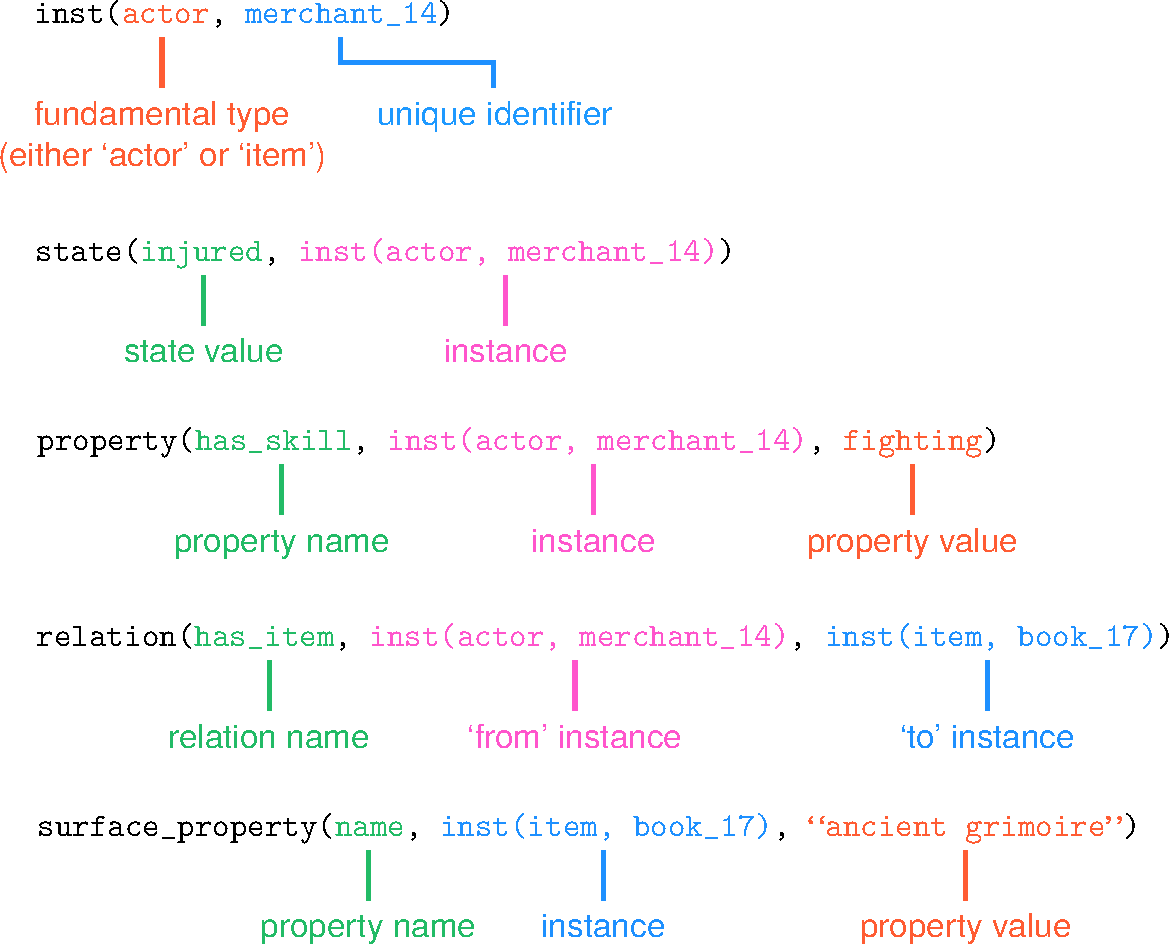
\includegraphics[width=\textwidth]{fig/cropped-dunyazad-states.pdf}
\caption[\dunyazad/'s state predicates]{Predicates used to describe states in \dunyazad/.}
\label{fig:dunyazad-states}
\end{figure}


The core states in \dunyazad/ describe the cast and any items or skills that those characters possess.
%
Beyond these states are a group of states that describe transient relationships which set the stage for action, these are called ``potentials.''
%
Potentials include things like \prq{knows\_gossip}{,} \prq{injured}{,} and \prq{threatening}{,} and each is classified as either a ``problem'' or an ``opportunity.''
%
Although these special potential states are represented using normal \prq{state}{,} \prq{property}{,} and \prq{relation}{} predicates, actions which get rid of them must specify whether each potential is \prq{resolved}{,} \prq{manifested}{,} or \prq{nullified}{.}
%
Additionally, extra predicates specify whether a potential is \prq{problematic\_for}{} one or more of the actors involved (for example, the \prq{injured}{} state is \prq{problematic\_for}{} any actor to which it is applied).


\dunyazad/ understands based on this information whether the action which eliminated a potential was good or bad for different characters.
%
For example, an action that \prq{resolves}{} an \prq{injured}{} state is good for the actor who was injured, and thus taking that action makes sense for that character.
%
States themselves thus directly encode some of the information used to decide which actions are viable.
%
This not only helps the system reason about motivation, but it also makes the design of actions and setups easier by providing a standard set of states that trigger certain actions.


\begin{figure}[!b]
\centering
\fbox{%
\parbox{0.9\textwidth}{
Scene:\svind\\
\ind ``A merchant carrying some perfume is being threatened by bandits.''\vind\\
Representation:\svind \\
\ind \parbox{0.9\textwidth}{ \tt
inst(actor,businessperson\_4). \\
inst(actor,tough\_3). \\
inst(item,treasure\_5). \\
property(type,inst(actor,businessperson\_4),merchant). \\
property(type,inst(actor,tough\_3),bandits). \\
property(type,inst(item,treasure\_5),perfume). \\
relation( \\
\ind has\_item, \\
\ind inst(actor,businessperson\_4), \\
\ind inst(item,treasure\_5) \\
). \\
relation( \\
\ind threatening, \\
\ind inst(actor,tough\_3), \\
\ind inst(actor,businessperson\_4) \\
). \\
surface\_property(name,inst(item,treasure\_5),"perfume").
}
}
}
\caption[\dunyazad/ state example]{An example scene description using \dunyazad/'s internal representation, showing the most-relevant predicates. In real output, each of these predicates except the \prq{surface\_property}{} would be tied to a specific timepoint, and there would be many more \prq{surface\_property}{} predicates describing things like the name of each instance and whether it is plural or singular. Note that each instance is assigned a unique identifier that ends with a number.}
\label{fig:dunyazad-state-example}
\end{figure}


\Cref{fig:dunyazad-state-example} is not quite accurate, because \dunyazad/'s non-surface state predicates are never encountered raw.
%
Instead, they are wrapped in \prq{st(<timepoint>, <state>)}{} predicates, to define different states of the world for each timepoint in the story.
%
The timepoints in a story form a directed acyclic graph that branches out from a single root node.
%
The structure of this graph is defined using \prq{successor(<previous>, <option>, <next>)}{} predicates which specify that the result of choosing option \prq{<opt>}{} at timepoint \prq{<previous>}{} is the state designated \prq{<next>}{.}
%
The root timepoint is named \prq{root}{,} and each successor is named for its parent plus the number of the option that leads to it, so for example, if there were three options at the \prq{root\_2}{} node, they would lead to timepoints labelled \prq{root\_2\_1}{,} \prq{root\_2\_2}{,} and \prq{root\_2\_3}{.}
%
The timepoints do not necessarily form a tree, however: if two outcomes lead to identical states, as long as it would not form a cycle in the graph, \dunyazad/ may connect them to the same timepoint.


\subsubsection{Actions}

As mentioned above, timepoints in \dunyazad/ are connected by options.
%
Each option is associated with a single action, and arguments describe the details of that action (for example, the initiator and/or target).
%
If a timepoint has more than one option, it represents a choice to be made by the player, otherwise it is simply an event that happens.
%
Actions specify lists of outcome variables with values for each variable.
%
For each outcome variable that an action has, a single outcome value is assigned to each option that uses that action, thereby defining the entire impact of that option on the world state.
%
These assignments have a shorthand notation \prq{o(<variable>, <value>)}{} which indicates that the outcome variable \prq{<variable>}{} takes on the value \prq{<value>}{.}
%
Each such assignment is an outcome component, and together, all such assignments for an action are the outcome of that action.
%
\Cref{fig:dunyazad-action-example} shows an example where at timepoint \prq{root}{,} the action associated with option 1 is \prq{talk\_down}{,} with two outcomes: \prq{o(attitude, convinced)}{} and \prq{o(enraged, not\_enraged)}{}.
%
Note that each outcome variable is responsible for deciding whether or not a particular state change occurs (or between several possible state changes one of which must occur).
%
The consequences of an action in terms of the world state are thus fully determined by the values its outcome variables.

\begin{figure}[!t]
\centering
\fbox{%
\parbox{0.9\textwidth}{
Option:\svind\\
\ind ``You try to talk the bandits down.''\vind \\
Outcome:\svind\\
\ind ``You talk to the bandits and convince them to back off.''\vind \\
Representation:\svind \\
\ind \parbox{0.9\textwidth}{ \tt
\cg{at(root,} action(option(1), talk\_down)\cg{).} \\

\cg{at(root,} arg(option(1), asking, inst(actor, you))\cg{).} \\
\cg{at(root,} arg(option(1), listening, inst(actor, tough\_3))\cg{).} \\
\cg{at(root,} arg(option(1), victim, \\
\ind inst(actor, businessperson\_4))\cg{).} \\

\cg{at(root,} outcome(option(1), o(attitude, convinced))\cg{).} \\
\cg{at(root,} outcome(option(1), o(enraged, not\_enraged))\cg{).} \\

\cg{at(root,} consequence\_of(option(1), o(attitude, convinced), \\
\ind \_not, relation(threatening, \\
\ind \ind inst(actor, tough\_3), inst(actor, businessperson\_4)))\cg{).} \\
\cg{at(root,} consequence\_of(option(1), o(enraged, enraged), \\
\ind \_not, relation(threatening, \\
\ind \ind inst(actor, tough\_3), inst(actor, you)))\cg{).} \\

\cg{at(root,} consequence(option(1), \\
\ind \_not, relation(threatening, \\
\ind \ind inst(actor, tough\_3), inst(actor, businessperson\_4)))\cg{).}
}
}
}
\caption[\dunyazad/ action example]{An example of action representation in \dunyazad/. Note that even outcomes which do not occur (\prq{o(enraged, enraged)}{} in this case) have their potential consequences noted via \prq{consequence\_of}{} predicates, but only outcomes that do occur (as specified by the \prq{at(<timepoint>, outcome(option(<opt>), o(<outvar>, <outval>)))}{} predicates) have actual consequences. }
\label{fig:dunyazad-action-example}
\end{figure}


Each action thus has multiple possible outcomes.
%
For the \prq{talk\_down}{} action, there are theoretically four: the \prq{attitude}{} outcome variable has two exclusive values \prq{convinced}{} and \prq{unconvinced}{,} while the \prq{enraged}{} outcome variable has two more values: \prq{enraged}{} and \prq{not\_enraged}{.}
%
However, the definition of \prq{talk\_down}{} stipulates that the outcome \prq{o(enraged, enraged)}{} is only possible if the outcome \prq{o(attitude, unconvinced)}{} is also present, so there are only three possibilities:

\begin{enumerate}
  \item The target is convinced to calm down (\prq{o(attitude, convinced)}{} and \prq{o(enraged, not\_enraged)}{}), in which case they stop threatening whoever they were threatening.
  \item The target is unconvinced, and nothing changes (\prq{o(attitude, unconvinced)}{} along with \prq{o(enraged, not\_enraged)}{}).
  \item The target is unconvinced, and gets mad at the person who tried to convince them (\prq{o(attitude, unconvinced)}{} along with \prq{o(enraged, enraged)}{}).
\end{enumerate}

Note that for a traditional planning system, because each combination of outcome variables has a different effect on the world state, each action would have to be broken into multiple sub-actions with fixed pre- and post-conditions.
%
The advantage of grouping them together conceptually is that this represents the player's view of things: the text introducing an option doesn't indicate the values of its outcome variables, and so the player can never be completely sure what outcomes an action will have.
%
This way of representing actions thus helps the system reason about how the player might perceive actions, this is the same reason that possible but unrealized state changes are explicitly represented by the system using \prq{consequence\_of}{} predicates (see \cref{fig:dunyazad-action-example}).


\begin{table}[!h]
\begingroup
\renewcommand*{\arraystretch}{1.5}
\begin{tabular}{c c c c}
  \pr{accuse}       & \pr{explain\_innocence} & \pr{play\_song}         & \pr{talk\_down} \\
  \cg{\pr{arrive}}       & \pr{flee}               & \pr{polymorph}          & \pr{tell\_story} \\
  \pr{attack}       & \pr{gossip}             & \cg{\pr{pursue}}             & \pr{trade} \\
  \pr{buy\_healing} & \pr{leave}              & \pr{reach\_destination} & \pr{travel\_onwards} \\
  \pr{deny\_blame}  & \pr{pacify}             & \pr{shift\_blame}       & \pr{treat\_injury} \\
  \pr{dispel}       & \pr{pay\_off}           & \pr{steal}
\end{tabular}
\endgroup
\caption[List of actions in \dunyazad/]{The 23 actions currently defined in \dunyazad/. The \prq{arrive}{} and \prq{pursue}{} actions aren't currently used because the system has no setups that motivate them.}
\label{tab:dunyazad-action-list}
\end{table}


Besides defining outcomes, actions also define how skills affect their outcomes, by asserting that certain outcome values are linked to the presence or absence of particular skills on the part of one or more participants of the action.
%
These links are denoted by \prq{skill\_link}{} predicates, and tools may also be involved.
%
For example the \prq{attack}{} action has an outcome variable \prq{success}{} with three values: \prq{victory}{,} \prq{defeat}{,} and \prq{tie}{.}
%
It specifies that the outcomes \prq{o(success, victory)}{} and \prq{o(success, defeat)}{} are both linked to the \prq{fighting}{} skill as alternate outcomes of a skill contest between the \prq{aggressor}{} and \prq{target}{} of the action, where tools are advantageous.
%
This means that if the aggressor of an attack action has both the \prq{fighting}{} skill and a tool for that skill, while the target of the attack has neither (or even if they're just missing a tool) the \prq{o(success, victory)}{} outcome is more likely, and the \prq{o(success, defeat)}{} outcome is less likely (the exact consequences of these assignments will be discussed in \cref{sec:dunyazad-poetic-constraints}).
%
Effectively, the definition of an action thus includes enough information for \dunyazad/ to consider both possible consequences of an action and what initial states might best foreshadow each different outcome.


\dunyazad/ currently has a total of 23 different actions, listed in \cref{tab:dunyazad-action-list}.
%
Given the setups that exist, however, the \prq{arrive}{} and \prq{pursue}{,}, actions are never motivated and thus impossible to use, so there are effectively 21 possible actions.
%
Most actions have at least two possible outcome configurations, and a few (such as \prq{attack}{}) have four or more.
%
However, the number of actions that are possible in a given state are limited by the constituent and aesthetic constraints.
%
This is where the setups come in: most actions require some sort of motivating state to make sense (the \prq{talk\_down}{} action, for example, requires that either a \prq{threatening}{} or an \prq{accusing}{} relationship be present).
%
Setups represent existing situations that the player might encounter while travelling, and each sets up conditions for a particular subset of actions.


\subsubsection{Setups}

Besides the initial state of the world having to do with the protagonist(s) and their starting skills and equipment, most of the state in \dunyazad/ comes from setups.
%
The situations \dunyazad/ creates are designed to fit into an overarching travel narrative: the protagonist(s) are on a journey, and encounter various obstacles.
%
This provides an excuse to repeatedly clean up the world state by having the main character(s) ``travel onwards,'' getting rid of any states except those pertaining to the main character(s) and introducing a new setup.
%
When putting multiple timepoints together into a complete branching story, \dunyazad/ starts by introducing a setup and then adding a few timepoints which resolve any outstanding potentials in that setup.
%
It then adds a \prq{travel\_onwards}{} option to each branch where potentials have been resolved, and adds a new setup to the timepoint that follows this option.


Setups are thus expected to set the stage for action: they provide a situation that contains the potential for something interesting to occur.
%
Some setups are quite flexible while others are specific.
%
For example, the \prq{healer}{} setup simply adds an actor with the \prq{healing}{} skill and a tool for healing who is offering to treat injuries for a price; it may only be used when a protagonist is injured.
%
In contrast, the \prq{market}{} setup potentially includes a lowlife, a healer, a laborer, an aristocrat, and up to two merchants.
%
These characters can have several potentials between them: the lowlife can be threatening one of the merchants, the noble might be accusing the peasant or one of the merchants, or perhaps the merchants are simply selling things and the noble or laborer knows some gossip.
%
The wide range of possibilities allowed by the \prq{market}{} setup lets \dunyazad/ create a variety of situations in service of creating particular choice structures, whereas the \prq{healer}{} setup is designed to be deployed in a very particular circumstance.
%
Although the \prq{market}{} setup eclipses the \prq{healer}{} setup in terms of actions enabled, the \prq{healer}{} setup's lack of extraneous characters provides a very different feeling to the player, and its surface text is more specific.


As mentioned above, not every timepoint includes setup-induced state changes: they only occur for the \prq{root}{} node and for timepoints that follow \prq{travel\_onwards}{} actions.
%
Internally, \dunyazad/ refers to everything that occurs between one setup and the \prq{travel\_onwards}{} events which follow that setup on each branch from it as a vignette.
%
The states associated with a setup are introduced after the \prq{travel\_onwards}{} action first removes all states associated with the old location---only states directly associated with a protagonist (such as an injury sustained or an item acquired) are retained.
%
Because \dunyazad/ effectively solves entire timepoints at once, however, the particular configuration of a setup's flexible elements can be changed at the same time that the actions, arguments, and outcomes of options are being decided.
%
This means that \dunyazad/ has the freedom to consider all possible setups as well as all configurations of actions given those setups when trying to build a particular choice structure, unless a certain setup is mandated by outside restrictions.


\subsection{Constituent Constraints}

\dunyazad/'s representation of stories as a graph of timepoints leaves lots of room for structures that don't make any sense.
%
This is where the constituent constraints come in.
%
While the basic predicates that define representational elements ensure things like continuity of states between timepoints, constituent constraints help ensure that actions get assembled into a story, instead of just a random sequence of unrelated events.
%
For example, rules that prohibit the same action from happening twice in a row,
or that require that each action be motivated, are constituent constraints.


While there is sometimes a gray area between constituent and aesthetic constraints, constituent constraints can often be identified as being concerned with getting \dunyazad/ to produce stories at all, while aesthetic constraints help defined \dunyazad/'s particular flavor of story.
%
If constituent constraints are removed, the results are often nonsensical; if aesthetic constraints are removed results still make sense, but they no longer fit with other stories that \dunyazad/ constructs.
%
\Cref{tab:dunyazad-constraints-inventory} lists all of the source code files from \dunyazad/'s main answer set problem definition code and briefly indicates what rules each file contains from each constraint type.

\begin{table}[!p]
\begin{minipage}[t][0.935\textheight]{\dimexpr0.5\textwidth-1.2em}
\begin{hangparas}{0.8em}{1}
\setlength{\parskip}{0.5em}
\file{actions.lp} \\
  \cg{[representational]} Action representation; consequences. \\
  \cg{[constituent]} Incapacitation. \\
  \cg{[poetic]} `Surprising' outcomes based on likely/unlikely outcomes.

\file{actors.lp} \\
  \cg{[representatonal]} Unpacking for actors; top level of actors ontology.

\file{choice\_structure.lp} \\
  \cg{[constituent]} Motivation; relevance; redundancy; repetition.  \\
  \cg{[aesthetic]} Narrative perspective (second-person); setup variety; bans boredom and trick options. \\
  \cg{[poetic]} Story length and pacing.

  \file{core.lp} \\
  \cg{[representational]} Basic structure (options, events, choices, etc.); exclusivity for states; reflexivity for actions; ontology basics (inheritance).

  \file{eval.lp} \\
  \cg{[poetic]} Expectations; stakes; option feels; option structures; outcome perceptions; outcome predictabilities; outcome feels.

  \file{goals.lp} \\
  \cg{[poetic]} Player goals; guilt.

  \file{grow.lp} \\
  \cg{[representational]} Timepoint ordering and links; timepoint creation and state transfer; state matching.

  \file{items.lp} \\
  \cg{[representational]} Unpacking for items; tool possession for skills; communal ownership for trading.
\end{hangparas}%
\end{minipage}%
\hfill
\noindent
\begin{minipage}[t][0.935\textheight]{\dimexpr0.5\textwidth-1.2em}
\begin{hangparas}{0.8em}{1}
\setlength{\parskip}{0.5em}
  \file{potential.lp} \\
  \cg{[representational]} Resolution methods, initiators, urgency/immediacy, and importance of potentials; unresolved and hidden potentials.

  \file{settings.lp} \\
  \cg{[content]} The possible settings. \\
  \cg{[representational]} Setting assign\-ment; setting continuity.

  \file{setup.lp} \\
  \cg{[representational]} Unpacking for setups; setup state creation.

  \file{skills.lp} \\
  \cg{[content]} The list of skills. \\
  \cg{[representational]} Relevance for skills and tools. \\
  \cg{[constituent]} Outcome likelihoods.

  \file{surface.lp} \\
  \cg{[representational]} Surface properties like names and genders.

  \file{the\_party.lp} \\
  \cg{[content]} Rules that define the starting state of the protagonist(s).

  \file{utils.lp} \\
  \cg{[other]} Helpers; name assignment.

  \file{vignettes.lp} \\
  \cg{[constituent]} Scoping of vignettes (actions in a single location).

  \file{content/*} \\
  \cg{[content]} These files define the actions, goals, potentials, and setups that \dunyazad/ can use, along with its ontology of actors and items.
\end{hangparas}%
\end{minipage}%
\caption[\dunyazad/ constraints inventory]{An inventory of \dunyazad/'s constraints organized by file and by constraint type.}
\label{tab:dunyazad-constraints-inventory}
\end{table}

The major topics covered by the constituent constraints are as follows:
%
\begin{itemize}
  \item Incapacitation---constraints that prevent injured actors from taking vigorous actions like fighting, and prevent dead actors from doing anything.
  \item Motivation---these constraints require that the actor that initiates each action have a motivation for taking that action.
  \item Relevance---constraints which require that actions address an existing important potential. These get rid of situations where someone fighting for their life might stop to buy fruit, for example.
  \item Redundancy---these constraints prevent two options at the same choice from being redundant.
  \item Repetition---these constraints prevent direct repetition: repeated actions at subsequent timepoints and repeated use of the same setup for subsequent vignettes.
  \item Outcome likelihoods---these constraints describe how skills and tools make certain outcomes more or less likely. Without them, outcomes would have no relation to the skills and tools of the participating actors.
  \item Vignette scoping---constraints that determine when \prq{travel\_onwards}{} actions are appropriate and thus where new setups should be applied.
\end{itemize}
%
Along with the representational constraints discussed above, these constituent constraints force answer sets to represent something that resembles a story, as opposed to a random mish-mash of incomprehensible actions.
%
The aesthetic constraints take things one step further and isolate a particular kind of story that \dunyazad/ tries to create.

\subsection{Aesthetic Constraints}

\dunyazad/'s aesthetic constraints go beyond the basics required to produce actions that make sense and can be read as a story and attempt to define what kind of stories \dunyazad/ will produce.
%
As shown in \cref{tab:dunyazad-constraints-inventory} there are several different categories:
%
\begin{itemize}
  \item Narrative perspective---these constraints require that all actions at choice points be initiated by the protagonist(s) and that all other actions are initiated by non-protagonists, effectively establishing a loose second-person narrative perspective.
  \item Setup variety---These constraints force \dunyazad/ to use a variety of setups over the course of a story, rather than just revisiting a few. This goes beyond prohibiting direct repetition and establishes a ``breadth'' requirement: before you can repeat a setup for the $n$th time, you must have used a total of at least $n+1$ unique setups (including the setup in question).
  \item Boredom---Beyond the repetition constituent constraints, these constraints target things like repeated failed attempts to solve the same problem, or the recurrence of a problem within a single scene. Although not something that would seem obviously broken to readers, these possibilities were deemed less interesting and prohibited.
  \item Trick options---If there are multiple protagonists and one has the skill necessary to perform a certain action while another lacks it, giving the player the option of having the unskilled protagonist perform that action is a kind of trick and this can feel very bad for the player as they're essentially not given the most rational option (which would be to have the skilled party member perform the action) but at the same time reminded of its presence. These constraints simply rule out this possibility, even though one could imagine using it for dramatic effect.
\end{itemize}


These aesthetic constraints are admittedly a bit underdeveloped.
%
In particular, there are not enough related to ensuring that long-term actions form a coherent plot, and this is one reason\footnote{A more important reason was the elimination of confounding factors.} that the experiments discussed in \cref{ch:results} focus on single choices rather than entire stories.
%
This is an open area of future work for \dunyazad/: developing stronger plot structures across multiple actions would allow it to produce interesting short stories and thus to support more complicated experiments.

\subsection{Poetic Constraints}
\label{sec:dunyazad-poetic-constraints}%

\dunyazad/'s poetic constraints are mechanisms for authorial control.
%
Together, they establish a set of predicates which can be required or forbidden in order to drive the creation of different kinds of choices.
%
These constraints are thus not about declaring what is universally acceptable or unacceptable, but rather about distinguishing between multiple interesting possibilities and providing the author the ability to make choices between these at a high level.
%
The bulk of these constraints form \dunyazad/'s operationalization of choice poetics, but a few are concerned with other effects:
%
\begin{itemize}
  \item Surprising outcomes---Using the notion of likely and unlikely outcomes based on skills and tools, \dunyazad/ labels outcomes which are deemed unlikely as `surprising.' In an earlier version, `surprising' outcomes were prohibited altogether, now it's up to the author whether or not to allow them.
  \item Story length and pacing---\dunyazad/ has rules for constraining how many actions must occur before a story ends, and how many of these must be choices as opposed to simple events.
\end{itemize}
%
Besides these two categories of constraint, \dunyazad/'s poetic constraints are focused on choice poetics, and in particular, implementing the goal-based choice analysis method described in \cref{sec:goal-based-choice-analysis} and illustrated in \cref{fig:choice-analysis-method}.
%
These constraints are the focus of the experiments described in \cref{ch:results} and they have been the focus of development on \dunyazad/ so far: these are the constraints that allow \dunyazad/ to attempt to create specific poetic effects when constructing choices.
%
Although the details of goal-based choice analysis were the main subject of \cref{ch:choice-poetics}, the following section provides a walk-through of \dunyazad/'s technical implementation of the technique.

\subsubsection{Choice Poetics}

\dunyazad/'s choice poetics constraints rely on a few underlying properties of its stories that were just discussed, most notably the concept of likely and unlikely outcomes based on skills and tools.
%
In \dunyazad/'s code it is assumed that players will be roughly aware of these things, and the surface text code does its best to ensure this.
%
If this assumption is violated, \dunyazad/'s choices may have unintended poetic effects, just as when an author fails to clearly communicate and leaves some of their audience confused.
%
Results so far seem to indicate that this assumption is mostly correct, however, so \dunyazad/'s conflation of its internal likelihoods with players' perceptions of such seems to be acceptable.


It is no accident that the breakdown of choice structures described in \cref{sec:cp-choice-representation} corresponds exactly to \dunyazad/'s internal representation of a choice as having an initial state, several options, and several outcomes at each option.
%
When a choice occurs directly after a setup (which always happens when \dunyazad/ generates a single choice) the setup becomes the framing.
%
The options are each a single action, described to the player before a choice is made without mention of any outcomes.
%
Once the player chooses, they see the outcome for the option they selected, which is a description of each outcome component (an \prq{o(<variable>, <value>)}{} pair) of that action.
%
The idea of potential outcomes also has a direct analogue: these are the other possible values of outcome variables for an action.


Each of the seven steps of choice analysis described in \cref{sec:goal-based-choice-analysis} has a corresponding set of rules in \dunyazad/ which depend on the rules for earlier steps:
%
\begin{enumerate}
\item %
\textbf{Goal Analysis} \\
%
This step is quite simple in \dunyazad/: the file \file{goals.lp} includes rules that directly state the player's goals in every situation.
%
Of course, forcing the author to estimate the player's goals like this is not perfect, but results so far indicate that it works tolerably well.
%
Individual content files that specify how each goal works provide rules for determining the priority of the goal in a given situation (this is binary, either `high' or `low').
%
These files also define at least one state that \prq{achieves}{,} \prq{fails}{,} \prq{hinders}{,} or \prq{advances}{} the goal.
%
For example, the \prq{preserve\_health}{} goal always has high priority and specifies that the states \prq{injured}{} and \prq{killed}{} both \prq{fail}{} the goal when true of the goal's target.
%
\file{goals.lp} then specifies that at every timepoint, the player has a \prq{preserve\_health}{} goal for each protagonist, allowing \dunyazad/ to understand that an action which might have an outcome that kills a protagonist will be viewed by the player as carrying some risk.
%
The full list of player goals assumed by the system is as follows:
%
\begin{itemize}
\item The player always has a \prq{preserve\_health}{} goal for each protagonist. As mentioned above, these goals are always high-priority and are failed by the \prq{injured}{} and \prq{killed}{} states.
\item The player always has an \prq{avoid\_threats\_to}{} goal for each protagonist. Actions which cause \prq{threatening}{} relationships with a protagonist as the object \prq{hinder}{} these goals, as do actions which allow such a state to persist (i.e., actions which don't have a consequence that resolves such a state when one exists). These goals are always high-priority.
\item The player always has an \prq{avoid\_accusations}{} goal for each protagonist. These goals work just like \prq{avoid\_threats\_to}{} goals but for the \prq{accusing}{} relationship, which indicates that someone is being accused of a crime. As with \prq{avoid\_threats\_to}{}, these goals are high-priority.
\item The player always has a \prq{preserve\_original\_form}{} goal for each protagonist. The \prq{polymorph}{} action represents a magic spell that can turn someone into a chicken; these goals assume that this is a state to be avoided an reversed whenever possible. These goals are high-priority.
\item Whenever an item has been stolen from a protagonist, the player has a \prq{reclaim\_property}{} goal for that item/protagonist. This goal is achieved when the \prq{has\_item}{} relation holds between the original owner and the item, and it it always high-priority.
\item The player always has an \prq{as\_intended}{} goal for each protagonist. These goals make use of the \prq{default\_intent}{} predicates specified in the definition of each action. Essentially, each action declares one or more outcome components to be its default intent: the outcome that the initiator of the action is hoping for. In the case of the \prq{attack}{} action, for example, the outcome component \prq{o(success, victory)}{} is a \prq{default\_intent}{}. When a \prq{default\_intent}{} outcome component is present, the \prq{as\_intended}{} goal of the action's initiator is achieved, when absent, the goal is failed. These goals are always low-priority, because they don't represent any particular bad or good states: there are many situations where an unintended outcome can be good for a character, and actual good or bad results are more important than things going as intended.
\item The player always has a \prq{have\_tool\_for}{} goal for each skill of each protagonist. These goals are achieved by possessing an item which counts as a tool for a particular skill, and they are always low-priority. The assumption that the player will have these goals is probably the weakest such, as players may not always remember at each moment what skills they have and which ones they have tools for. However, the presence of these goals means that trading items for goods or services can have value, and they can differentiate good trades from bad ones. In situations where players had a chance to play multiple stories, players would be more likely to consider these goals when making choices.
\item The final goals assigned to the player presume that players are generally sympathetic: unless a character is actively threatening or accusing another (deemed `guilty' by the system), the player is assumed to have both \prq{avoid\_threats\_to}{} and \prq{avoid\_accusations}{} goals for that character. These goals mean that when the player encounters non-protagonists threatening or accusing each other, the system assumes that the player will want to help the victim. As above, these goals are high-priority.
\end{itemize}
%
The predicates created by \file{goals.lp} are \prq{at(\abr/<timepoint>,\abr/ player\_goal(\abr/<goal>))}{} predicates which specify the goals of the player for each timepoint, and \prq{at(\abr/<timepoint>,\abr/ goal\_stakes(\abr/<goal>,\abr/ <priority>))}{} predicates which assign priorities to each goal.


Although this static goal analysis works reasonably well, an interesting opportunity for future work presents itself here.
%
Not only could \dunyazad/ benefit from dynamic goal analysis (perhaps along the lines of the user model used for dilemma generation in \citep{Barber2007b}), as a system that produces choice-based narratives, it could incorporate explicit choices-of-goals as part of the stories it generates, and use the results of these choices as direct statements of player intent rather than relying on authorial guesswork.
%
This would require a major overhaul of the goals system, however, and goals might have to be represented as mutable states of the world, which would place an additional burden on the solver.

\label{sec:dunyazad-modes-of-engagement}%
One thing that should be mentioned here is that \dunyazad/'s goal assumptions are targeted at players whose mode of engagement is a mix of avatar and power play.
%
There are no goals related to character believability of the protagonist, nor are there goals related to things like curiosity.
%
These could in principle be declared just like the current goals, but \dunyazad/ focuses on avatar and power play because these are the modes that its genre traditionally encourages.

\item %
\textbf{Likelihood Analysis} \\
%
This step is already performed by \dunyazad/'s constituent constraints, using the \prq{skill\_link}{} predicates supplied by action definitions along with information on the skills and tools available to the actors involved in each action. 
%
Recall that individual outcome components are labelled as likely or unlikely, rather than entire outcomes, as called for in \cref{sec:goal-based-choice-analysis}.
%
This step produces the \prq{at(\abr/<timepoint>,\abr/ likely\_outcome(\abr/<option>,\abr/ <outcome>))}{} and \prq{at(\abr/<timepoint>,\abr/ unlikely\_outcome(\abr/<option>,\abr/ <outcome>))}{} predicates.

\item %
\textbf{Option Analysis} \\
\label{page:option-analysis}%
%
As explained in \cref{sec:goal-based-choice-analysis}, the option analysis step uses the results of goal and likelihood analysis to attach expectations to each option.
%
In the code, goal predicates specify which state(s) affect them, and the likelihood of all possible outcomes is known, so option analysis is straightforward.
%
First, all possible outcome components of an option are considered and if any of them has a negative consequence for a goal, that option \lbl{threatens} that goal.
%
Similarly, any positive consequence entails an \lbl{enables} relationship (the \prq{threatens}{} and \prq{enables}{} predicates in the code are used for the \lbl{threatens} and \lbl{enables} labels from \cref{ch:choice-poetics}).
%
Since each option has multiple outcome components, a single goal may be both threatened and enabled by the same option, of course.
%
For the \lbl{advances} and \lbl{hinders} evaluations (represented in code by \prq{achieves}{} and \prq{fails}{} predicates), the same analysis applies, but only outcome components marked as \prq{likely}{} are considered.
%
The result of the option analysis constraints is a set of \prq{at(\abr/<timepoint>,\abr/ expectation(\abr/<option>,\abr/ <expectation>,\abr/ <goal>))}{} that list the expectations for each option/goal pair.

\item %
\textbf{Relative Option Analysis} \\
%
Integrating goal priorities and option expectations, relative option analysis produces \prq{at(\abr/<timepoint>,\abr/ option\_feel(\abr/<option>,\abr/ <feel>))}{} predicates, which collapse the various expectations across goals at each option to produce a general evaluation of that option.
%
For example, if an option has at least one \prq{achieves}{} expectation and it has no \prq{threatens}{} or \prq{fails}{} expectations across all goals (only counting goals tied for highest priority at that option) an option is labeled as a \prq{sure\_\abr/thing}{.}
%
These rules establish one or more \prq{option\_\abr/feel}{}s for each option, and these are further aggregated into \prq{option\_\abr/structure}{} assignments, which are the prospective impressions show in \cref{tab:prospective-impressions}.
%
These prospective impression assignments were the subject of the first experiment described in \cref{ch:results} and provide one primary means of controlling the kinds of choices \dunyazad/ generates.
%
Although they are discussed here as being `assigned' based on existing choice structures, because they're just predicates in an answer set program, they can be required and the solver will solve for answer sets that include them.
%
Requiring these \prq{option\_\abr/structure}{} predicates thus allows an author (or experimenter) to generate choices that (hopefully) make a desired prospective impression on the player.

\item %
\textbf{Outcome Component Analysis} \\
%
Using player goal information and information about all possible outcomes of each action, outcome component analysis maps the relationships between every possible outcome component and each goal.
%
These relationships have four basic values, similar to the \prq{expectation}{} predicates generated by the option analysis step: \prq{advances}{,} \prq{hinders}{,} \prq{achieves}{,} and \prq{fails}{.}
%
These are directly deduced from the definitions of each goal combined with the states that a particular outcome component adds or removes.
%
So for example, the \prq{o(\abr/success,\abr/ dispelled)}{} possible outcome component of the \prq{dispel}{} action has a consequence which removes the \prq{polymorphed}{} property from the target of the action.
%
Because of this, any option that consists of a \prq{dispel}{} action with a polymorphed target will \prq{advance}{} the \prq{preserve\_\abr/original\_\abr/form}{} goal for the target actor, (because the \prq{polymorphed}{} state which is being removed \prq{fails}{} the \prq{preserve\_\abr/original\_\abr/form}{} goal).

Because of the way that goals are defined in \dunyazad/ this step of analysis is fairly trivial.
%
Of course, not all goals are simple to define in terms of a globally applicable set of states that triggers them.
%
For example, the \prq{as\_\abr/intended}{} goal deals directly with outcomes as opposed to world states, which may be different depending on the context of an action.
%
Because of this, the \prq{as\_\abr/intended}{} goal definition has custom code which directly creates \prq{expectation}{} and \prq{outcome\_\abr/perception}{} predicates by considering which outcomes are likely (and which is the \prq{default\_\abr/intent}{,} as mentioned above).
%
The \prq{avoid\_\abr/accusations}{} and \prq{avoid\_\abr/threats\_\abr/to}{} goals also have a bit of custom code to make them more urgent: when an accusation or threat state is present, actions which have no effect on that state are given \prq{fails}{} expectations and \prq{hinders}{} outcome perceptions.
%
All other goals simply specify one or more states that \prq{advance}{,} \prq{hinder}{,} \prq{achieve}{,} or \prq{fail}{} them, as described above.

\item %
\textbf{Full Outcome Analysis} \\
%
Full outcome analysis concerns the expectedness and overall valence of the entire outcome of each option.
% TODO: Figure out how to do this non-manually!
In \dunyazad/, these are represented by the predicates \prq{at(\abr/<timepoint>,\abr/ outcome\_overall(\abr/<option>,\abr/ <evaluation>\abr/))}{,} \prq{at(\abr/<timepoint>,\abr/ outcome\_predictability(\abr/<option>,\abr/ <outcome>,\\ <predictability>))}{,} and \prq{at(\abr/<timepoint>,\abr/ overall\_predictability(\\ <option>,\abr/ <predictability>))}{.}
%
The \prq{outcome\_\abr/overall}{} predicates summarize the individual \prq{outcome\_\abr/perception}{} predicates across all player goals and across different outcome components at an action.
%
There are eight possible \prq{outcome\_\abr/overall}{} values:
%
\begin{enumerate}
\item \prq{great}{}---Reserved for options which achieve at least one player goal while neither failing nor hindering any.
\item \prq{good}{}---Options which would be \prq{great}{}, except that they merely advance at least one player goal as opposed to achieving any.
\item \prq{tradeoff}{}---Options which both achieve one goal and fail another, or which both advance one goal and hinder another (without either achieving or failing any).
\item \prq{worth\_it}{}---Options where the best outcome achieves a goal, but the worst outcome hinders a (presumably different) goal.
\item \prq{not\_worth\_it}{}---Options where the worst outcome fails a goal, while the best outcome advances a goal.
\item \prq{bad}{}---Options where no goals are achieved or advanced, and the worst outcome hinders a goal.
\item \prq{awful}{}---\prq{bad}{} options where a goal is failed instead of merely hindered.
\item Neutral---Options where no outcome is relevant to any player goal.
\end{enumerate}
%
Note that for all of these evaluations, only top-priority goals are considered (i.e., if there is at least one high-priority goal, only high-priority goals count; if not then low-priority goals can come into play).
%
Summarizing the potentially complex per-outcome-component evaluations from the outcome component analysis step like this helps make the retrospective analysis more tractable (both for humans and for the solver).
%
Most common cases avoid the ambiguous ``tradeoff'' label anyways, so not much information is lost.

Along with \prq{outcome\_\abr/overall}{} labels, this step assigns one of the following six \prq{outcome\_\abr/predictability}{} values to each outcome component and also (as \prq{overall\_\abr/predictability}{}) to each option:
%
\begin{enumerate}
\item
%
\prq{predictable}{}---An outcome component is \prq{predictable}{} when its value is the sole likely value for its variable.
%
An entire option is \prq{predictable}{} when every single important outcome component (an outcome component that affects one or more goals tied for the highest priority) is \prq{predictable}{}, and there is at least one such outcome component.
%
\item \prq{expected}{}---An outcome component is \prq{expected}{} when it is one of several likely values for its variable.
%
An entire option is \prq{expected}{} when every outcome at that option is either \prq{predictable}{,} \prq{expected}{,} or \prq{average}{,} and they're not \emph{all} \prq{average}{} (nor are all components unimportant).
%
\item \prq{average}{}---These outcome components aren't likely, but neither are they unlikely, and no other values for their variable are likely, while at least one is unlikely.
%
In other words, an outcome component is \prq{average}{} when a variable avoids an unlikely value but the value that it takes on isn't deemed likely.
%
An entire option is \prq{average}{} if every one of its important outcome components is average, and it has at least one important outcome.

\item \prq{unpredictable}{}---An outcome component is \prq{unpredictable}{} if for its variable, there are no likely or unlikely values, or if all values for its variable are unlikely.
%
An option as a whole is \prq{unpredictable}{} if it has at least one \prq{unpredictable}{} component and no \prq{unexpected}{} or \prq{unfair}{} components (counting only important outcome components).
\item \prq{unexpected}{}---An \prq{unexpected}{} outcome component is one where an \prq{unlikely}{} value is selected despite the presence of at least one \prq{neutral}{} value, but no actually \prq{likely}{} values are possible.
%
For an option to be labeled \prq{unexpected}{} as a whole, it must have at least one important \prq{unexpected}{} component and no \prq{unfair}{} components.
\item \prq{unfair}{}---An \prq{unfair}{} option component is one where an \prq{unlikely}{} value has been selected for a variable over a possible \prq{likely}{} value.
%
Every option that has an important \prq{unfair}{} outcome component is considered \prq{unfair}{} as a whole.
\end{enumerate}

There are actually two other predictability values that are used only for entire options: \prq{irrelevant}{} (used for options that are entirely lacking in \prq{outcome\_perception}{} predicates) and \prq{unrecognized}{} (used as a catch-all for situations that don't fit any other label).
%
As with the \prq{outcome\_overall}{} summarization, building \prq{overall\_predictability}{} predicates reduces the complexity of possible \prq{outcome\_predictability}{} configurations to a few cases which cover common situations.
%
In the same way that this is useful for efficient analysis (and more detailed analysis is always possible when necessary), it is helpful when authoring constraints (and likewise, constraints directly targeting complex \prq{outcome\_predictability}{} situations can be written if necessary).
%
The \prq{outcome\_overall}{} and \prq{overall\_predictability}{} predicates from this step are used alongside the \prq{outcome\_feel}{} predicates from relative option analysis as inputs for retrospective analysis.


\begin{table}[!p]
\begingroup
\renewcommand*{\arraystretch}{1.5}
{
\centering
\begin{tabular}{p{10em} p{6.5em} p{7.5em} p{6em}}
\toprule
\vspace{-1.5ex}\textbf{Outcome Feel}%
& \vspace{-1.5ex}\textbf{Option Feels}%
& \textbf{Overall \newline Predictabilities}%
& \textbf{Overall \newline Outcomes} \\
\midrule
\prq{expected\_success}{}%
& \prq{sure\_thing}{} \newline \prq{safe}{} \newline \prq{hopeful}{}%
& \prq{predictable}{} \newline \prq{expected}{}%
& \prq{great}{} \newline \prq{good}{} \\
\midrule
\prq{unfair}{}%
& \prq{sure\_thing}{} \newline \prq{safe}{} \newline \prq{hopeful}{}%
& \prq{unexpected}{} \newline \prq{unfair}{}%
& \prq{bad}{} \newline \prq{awful}{} \\
\midrule
\prq{nice\_gamble}{}%
& \prq{risky}{} \newline \prq{tradeoff}{} \newline \prq{irrelevant}{}%
& \prq{average}{} \newline \prq{unpredictable}{}%
& \prq{great}{} \newline \prq{good}{} \newline \prq{worth\_it}{} \\
\midrule
\prq{bad\_gamble}{}%
& \prq{risky}{} \newline \prq{tradeoff}{} \newline \prq{irrelevant}{}%
& \prq{average}{} \newline \prq{unpredictable}{}%
& \prq{not\_worth\_it}{} \newline \prq{bad}{} \newline \prq{awful}{} \\
\midrule
\prq{expected\_failure}{}%
& \prq{long\_shot}{} \newline \prq{bad}{} \newline \prq{doomed}{}%
& \prq{predictable}{} \newline \prq{expected}{} \newline \prq{average}{}%
& \prq{bad}{} \newline \prq{awful}{} \\
\midrule
\prq{miracle}{}%
& \prq{long\_shot}{} \newline \prq{bad}{} \newline \prq{doomed}{}%
& \prq{unexpected}{} \newline \prq{unfair}{}%
& \prq{great}{} \newline \prq{good}{} \newline \prq{worth\_it}{} \\
\bottomrule
\end{tabular}
}
\endgroup
\caption[Outcome feel structures]{%
  \dunyazad/'s six outcome feel structures.
  %
  If at least one of each of the given \prq{option\_feel}{,} \prq{overall\_predictability}{,} and \prq{outcome\_overall}{} values applies to an option, the listed \prq{outcome\_feel}{} applies.
  %
  For example, if a choice has a \prq{safe}{} \prq{option\_feel}{,} a \prq{predictable}{} \prq{overall\_predictability}{,} and a \prq{good}{} \prq{outcome\_overall}{}, then it meets the criteria for having the \prq{expected\_success}{} outcome feel.
}
\label{tab:dunyazad-outcome-feel-structures}
\end{table}

\item %
\textbf{Retrospective Analysis} \\
%
By comparing outcomes with option feels, an overall impression of a choice can be obtained.
%
These are represented using \prq{at(<timepoint>, outcome\_feel(<option>, <feel>))}{} predicates.
%
\dunyazad/ has six different \prq{outcome\_feel}{} structures that it recognizes, which are shown in \cref{tab:dunyazad-outcome-feel-structures}.


It's worth noting that contrary to \cref{fig:choice-analysis-method}, \dunyazad/ doesn't directly incorporate information from its option analysis step into its retrospective analysis.
%
This is because it doesn't use this more nuanced information, just using the higher-level \prq{outcome\_overall}{} predicates.
%
This connects to a deeper point: as a tool for automated \emph{analysis} of choices, \dunyazad/ would not perform very well, because its definitions are intentionally narrow.
%
The reason for this is twofold: first, broad definitions are harmful during generation, because they make it easier to produce things which don't actually fit the categories they are supposed to represent.
%
Second, scope and to some degree breadth of definitions was limited by effort---with more work, these could be improved.
%
Because of these limitations, \dunyazad/'s formal definitions of various properties are designed to be sufficient, but never necessary conditions for the effects they describe.
%
In other words, they are idiosyncratic: \dunyazad/'s definition of an `obvious' choice might be one way to make choices obvious, but there could be other rules for constructing choices that also resulted in obviousness without necessarily having any overlap with the kinds of obvious choices that \dunyazad/ generates.
%
Their idiosyncrasy is not a problem, of course: we can still learn about obviousness from studying a subset of obvious choices.
%
However, we need to be careful not to generalize our results too far.


Coming back to the results of retrospective analysis, these \prq{outcome\_feel}{} predicates give authors another high-level means of control over \dunyazad/.
%
As with the \prq{option\_feel}{} predicates, constraints requiring the presence of a particular \prq{outcome\_feel}{} force \dunyazad/ to produce choices that include such options (if it can), and this is how the second experiment described in \cref{ch:results} was set up.

\end{enumerate}


As is hopefully clear from this description, \dunyazad/'s poetic constraints are a direct mirror of the analysis method presented in \cref{sec:goal-based-choice-analysis}.
%
Although they operate simultaneously rather than sequentially, each step of analysis shown in \cref{fig:choice-analysis-method} corresponds to a set of constraints in \dunyazad/'s ASP code.
%
Of course, this is not simply a case of the code mimicking the theory: both the human-usable analysis method and the machine-usable code were designed together, with changes in each informing the development of the other.
%
Furthermore, the close parallels provided, which extend to the structural level, make this two-way information flow smoother, allowing both bug fixes to the code and caveats added to the theory to inform each other.

\section{High-Level Control}
\label{sec:dunyazad-control}%

\dunyazad/'s ASP rules allow it to represent an entire story without any trouble, but the complexity of the problem of generating an answer set when all elements of a story are left unconstrained is prohibitive.
%
In theory, \dunyazad/'s rules allow an entire story's worth of content to be solved for, but in practice, given the exponential runtime complexity of the solving algorithm and the size of the problems that \dunyazad/ can create, this is impractical.
%
Some simple statistics illustrate this: when asked to generate a single ``relaxed'' choice, \dunyazad/ produced a problem with 1,066,956 atoms and 24,974,521 rules, according to the output of \prog{clasp --stats}.
%
The grounded output for this problem was 994,932 lines of code; a total of 3.5 gigabytes of data (albeit in a relatively memory-inefficient format for human readability).
%
Grounding and finding the first answer set for this problem took almost 24 seconds of CPU time on a modern Intel i7 laptop with 12 gigabytes of RAM.
%
Even given \dunyazad/'s simple target genre, a full story would contain dozens to hundreds of nodes because of branching, and asking the solver to tackle that all at once is clearly out of the question.


The solution to this problem was to add a higher-level control layer that would ask the answer set solver to solve just one node at a time.
%
This layer keeps track of all of the answer sets received and integrates the parts of them that represent story content into a running predicate representation of the entire story, which is fed into every solver query.
%
This means that even though each ASP task can only make changes to one timepoint at once, it can see the entire story so far, and can take that information into account.
%
Adding many nodes as fixed constraints like this doesn't cost extra time; in fact, it usually saves time because the constraints added can make a solution easier to find for the solver (in particular, solving the first timepoint of a new vignette which necessarily involves a setup is much slower than solving intermediate timepoints which just play out action that has already been initiated).
%
The high-level control even goes a step further: the process of filling in information for a timepoint is actually split into four independent steps that can be processed separately (although at a slight cost, since choices in separately-processed steps can no longer affect each other).
%
The four steps for filling in a timepoint are defined in the file \file{grow.lp}:
\begin{enumerate}
  \item \prq{initialize\_node}{}---This phase involves choosing a setup for the target timepoint if necessary and locking down the starting state of the timepoint, including any changes introduced by the chosen setup. Player goals for a timepoint can also be discovered during this phase. Values for any variable elements of a setup must be chosen during this phase.
  \item \prq{build\_options}{}---The bulk of \dunyazad/'s constraints are tied to this phase, which solves for the options and outcomes at a timepoint.
  \item \prq{add\_branch\_nodes}{}---This phase adds successor links to the target timepoint and creates new successor timepoints if necessary. It's also responsible for transferring state between timepoints. The only decisions made during this phase are whether or not two branches which have exactly equivalent world states should link to the same timepoint or to two different timepoints, so running it separately loses little.
  \item \prq{add\_surface}{}---This phase doesn't change any of the essential facts of the story, but merely adds \prq{surface\_property}{} predicates and the like for the convenience of the English generation code. There are currently no constraints that link surface properties to story world state, so there is no cost associated with running this phase separately.
\end{enumerate}

Although four phases are defined, the control code actually makes a compromise for the sake of greater flexibility and only runs two separate problems per timepoint.
%
First, the \prq{initialize\_node}{} and \prq{build\_options}{} phases are run together, so that choices about setup variables can be influenced by choices about actions and their outcomes and vice versa.
%
Next, the \prq{add\_branch\_nodes}{} and \prq{add\_surface}{} phases are run together, which usually takes a fraction of the time taken by the other two phases.


Using two steps per node, the high-level code first fills in the root node of a story and then proceeds to randomly select an empty leaf timepoint to fill in, followed by random selection of an unbranched node to add branches to, and so on, until either there are no more branches left (because each has hit an ending) or a time- or story-size-limit is reached.
%
By proceeding in this manner, the high-level control code can solve for a story with dozens of nodes in a matter of minutes.
%
Of course, there is a sacrifice associated with this: it separates decisions about different timepoints, meaning that later timepoints must always do their best with the constraints placed on them by the past.
%
In practice, \dunyazad/ may even become stuck, when an authorial constraint (such as ``make all choices relaxed'') combines with accumulated state to create an unsatisfiable problem.
%
With \dunyazad/'s current design this happens quite rarely, so a backup procedure (perhaps deleting the unsatisfiable node and several of its parents before retrying) has not been necessary.
%
It would of course be possible to implement full back-tracking search at the higher level if conflicts were frequent, although the cost per timepoint instantiated (currently in the tens of seconds) would seem to suggest a search for alternative solutions.


As mentioned previously, \dunyazad/'s high-level control code is written in Python (version 3.x).
%
Besides the simple iterative process just described, there is code for managing constraint sets to be fed into the solver during each run (including extracting just the story predicates from previous runs), running the solver via the command line and capturing and parsing its output, and feeding the results into the English generation code.
%
Along with classes for representing predicates and answer sets, a full parser for \prog{clasp}'s output is included, although it is a bit slow and could do with more optimization.
%
For situations like the experiments described in \cref{ch:results}, there are also mechanisms for inserting extra constraints that will be used during every call to the solver.
%
Ultimately, the high-level Python code is relatively straightforward, with the exception of the English generation code.
%
Although \dunyazad/ generates English text using a somewhat sophisticated template-based system, the inner workings of that system (beyond its basic function of expressing predicate story representations as English text) are not critical to \dunyazad/'s function as a choice point generator.
%
Those interested can find a description of the template-based text generator that \dunyazad/ uses in \cref{ap:nlg}.


\section{Summary}

No project of \dunyazad/'s scope (modest though it may be) can be perfectly described in a technical write-up.
%
There are details that were left out or glossed over in the sections above, and to thoroughly understand how \dunyazad/ works down to the smallest details reading its source code is unavoidable.
%
% TODO: HERE link to source code in archival format as well as on github!
%
Luckily, such deep understanding should be unnecessary for most scholars who want to take something away from this work.
%
The choice analysis method presented in the \cref{ch:choice-poetics}, for example, does not depend on the intricate details of \dunyazad/ for its validity, although it may have undiscovered caveats which could be revealed by a careful inspection of \dunyazad/'s code.


Another reason that the description of \dunyazad/ given here can be appreciated on its own is that it describes all of the driving principles behind \dunyazad/'s inner workings, in enough detail for someone else to construct their own working system that generates narrative choices.
%
Technical considerations (such as iterative vs. all-at-once story construction) aside, the principles driving \dunyazad/ are not terribly complicated: a story representation that includes the concept of choices and actions with variable consequences along with systems for estimating what the player will think of these things.
%
One could re-implement it using an entirely different theory of choice poetics, for example, or without using logic programming at all.


From the perspective of generative systems, \dunyazad/ makes the statement: ``Generating narrative choices intentionally is computationally tractable, and here's one way to do it.''
%
Ideally this chapter is a convincing demonstration of that, but \dunyazad/ has ambitions well beyond being a working generative system.
%
In \cref{ch:results}, I will discuss the results of two experiments that both demonstrate \dunyazad/'s capabilities as a generative system and provide useful insight into choice poetics by leveraging its capacity as a tool for theory development.

\label{sec:dunyazad-summary}%
